% Options for packages loaded elsewhere
\PassOptionsToPackage{unicode}{hyperref}
\PassOptionsToPackage{hyphens}{url}
%
\documentclass[
]{article}
\usepackage{lmodern}
\usepackage{amssymb,amsmath}
\usepackage{ifxetex,ifluatex}
\ifnum 0\ifxetex 1\fi\ifluatex 1\fi=0 % if pdftex
  \usepackage[T1]{fontenc}
  \usepackage[utf8]{inputenc}
  \usepackage{textcomp} % provide euro and other symbols
\else % if luatex or xetex
  \usepackage{unicode-math}
  \defaultfontfeatures{Scale=MatchLowercase}
  \defaultfontfeatures[\rmfamily]{Ligatures=TeX,Scale=1}
\fi
% Use upquote if available, for straight quotes in verbatim environments
\IfFileExists{upquote.sty}{\usepackage{upquote}}{}
\IfFileExists{microtype.sty}{% use microtype if available
  \usepackage[]{microtype}
  \UseMicrotypeSet[protrusion]{basicmath} % disable protrusion for tt fonts
}{}
\makeatletter
\@ifundefined{KOMAClassName}{% if non-KOMA class
  \IfFileExists{parskip.sty}{%
    \usepackage{parskip}
  }{% else
    \setlength{\parindent}{0pt}
    \setlength{\parskip}{6pt plus 2pt minus 1pt}}
}{% if KOMA class
  \KOMAoptions{parskip=half}}
\makeatother
\usepackage{xcolor}
\IfFileExists{xurl.sty}{\usepackage{xurl}}{} % add URL line breaks if available
\IfFileExists{bookmark.sty}{\usepackage{bookmark}}{\usepackage{hyperref}}
\hypersetup{
  pdftitle={Instructions for Bottom-Up Decarbonization Policy Analysis},
  hidelinks,
  pdfcreator={LaTeX via pandoc}}
\urlstyle{same} % disable monospaced font for URLs
\usepackage[margin=1in]{geometry}
\usepackage{color}
\usepackage{fancyvrb}
\newcommand{\VerbBar}{|}
\newcommand{\VERB}{\Verb[commandchars=\\\{\}]}
\DefineVerbatimEnvironment{Highlighting}{Verbatim}{commandchars=\\\{\}}
% Add ',fontsize=\small' for more characters per line
\usepackage{framed}
\definecolor{shadecolor}{RGB}{248,248,248}
\newenvironment{Shaded}{\begin{snugshade}}{\end{snugshade}}
\newcommand{\AlertTok}[1]{\textcolor[rgb]{0.94,0.16,0.16}{#1}}
\newcommand{\AnnotationTok}[1]{\textcolor[rgb]{0.56,0.35,0.01}{\textbf{\textit{#1}}}}
\newcommand{\AttributeTok}[1]{\textcolor[rgb]{0.77,0.63,0.00}{#1}}
\newcommand{\BaseNTok}[1]{\textcolor[rgb]{0.00,0.00,0.81}{#1}}
\newcommand{\BuiltInTok}[1]{#1}
\newcommand{\CharTok}[1]{\textcolor[rgb]{0.31,0.60,0.02}{#1}}
\newcommand{\CommentTok}[1]{\textcolor[rgb]{0.56,0.35,0.01}{\textit{#1}}}
\newcommand{\CommentVarTok}[1]{\textcolor[rgb]{0.56,0.35,0.01}{\textbf{\textit{#1}}}}
\newcommand{\ConstantTok}[1]{\textcolor[rgb]{0.00,0.00,0.00}{#1}}
\newcommand{\ControlFlowTok}[1]{\textcolor[rgb]{0.13,0.29,0.53}{\textbf{#1}}}
\newcommand{\DataTypeTok}[1]{\textcolor[rgb]{0.13,0.29,0.53}{#1}}
\newcommand{\DecValTok}[1]{\textcolor[rgb]{0.00,0.00,0.81}{#1}}
\newcommand{\DocumentationTok}[1]{\textcolor[rgb]{0.56,0.35,0.01}{\textbf{\textit{#1}}}}
\newcommand{\ErrorTok}[1]{\textcolor[rgb]{0.64,0.00,0.00}{\textbf{#1}}}
\newcommand{\ExtensionTok}[1]{#1}
\newcommand{\FloatTok}[1]{\textcolor[rgb]{0.00,0.00,0.81}{#1}}
\newcommand{\FunctionTok}[1]{\textcolor[rgb]{0.00,0.00,0.00}{#1}}
\newcommand{\ImportTok}[1]{#1}
\newcommand{\InformationTok}[1]{\textcolor[rgb]{0.56,0.35,0.01}{\textbf{\textit{#1}}}}
\newcommand{\KeywordTok}[1]{\textcolor[rgb]{0.13,0.29,0.53}{\textbf{#1}}}
\newcommand{\NormalTok}[1]{#1}
\newcommand{\OperatorTok}[1]{\textcolor[rgb]{0.81,0.36,0.00}{\textbf{#1}}}
\newcommand{\OtherTok}[1]{\textcolor[rgb]{0.56,0.35,0.01}{#1}}
\newcommand{\PreprocessorTok}[1]{\textcolor[rgb]{0.56,0.35,0.01}{\textit{#1}}}
\newcommand{\RegionMarkerTok}[1]{#1}
\newcommand{\SpecialCharTok}[1]{\textcolor[rgb]{0.00,0.00,0.00}{#1}}
\newcommand{\SpecialStringTok}[1]{\textcolor[rgb]{0.31,0.60,0.02}{#1}}
\newcommand{\StringTok}[1]{\textcolor[rgb]{0.31,0.60,0.02}{#1}}
\newcommand{\VariableTok}[1]{\textcolor[rgb]{0.00,0.00,0.00}{#1}}
\newcommand{\VerbatimStringTok}[1]{\textcolor[rgb]{0.31,0.60,0.02}{#1}}
\newcommand{\WarningTok}[1]{\textcolor[rgb]{0.56,0.35,0.01}{\textbf{\textit{#1}}}}
\usepackage{longtable,booktabs}
% Correct order of tables after \paragraph or \subparagraph
\usepackage{etoolbox}
\makeatletter
\patchcmd\longtable{\par}{\if@noskipsec\mbox{}\fi\par}{}{}
\makeatother
% Allow footnotes in longtable head/foot
\IfFileExists{footnotehyper.sty}{\usepackage{footnotehyper}}{\usepackage{footnote}}
\makesavenoteenv{longtable}
\usepackage{graphicx,grffile}
\makeatletter
\def\maxwidth{\ifdim\Gin@nat@width>\linewidth\linewidth\else\Gin@nat@width\fi}
\def\maxheight{\ifdim\Gin@nat@height>\textheight\textheight\else\Gin@nat@height\fi}
\makeatother
% Scale images if necessary, so that they will not overflow the page
% margins by default, and it is still possible to overwrite the defaults
% using explicit options in \includegraphics[width, height, ...]{}
\setkeys{Gin}{width=\maxwidth,height=\maxheight,keepaspectratio}
% Set default figure placement to htbp
\makeatletter
\def\fps@figure{htbp}
\makeatother
\setlength{\emergencystretch}{3em} % prevent overfull lines
\providecommand{\tightlist}{%
  \setlength{\itemsep}{0pt}\setlength{\parskip}{0pt}}
\setcounter{secnumdepth}{-\maxdimen} % remove section numbering
\usepackage{mathptmx}
\usepackage[version=4]{mhchem}

\newcommand{\COO}{\ce{CO2}}
\newcommand{\methane}{\ce{CH4}}
\newcommand{\degC}{^\circ \mathrm{C}}
\newcommand{\degF}{^\circ \mathrm{F}}
\newcommand{\water}{\mathrm{H_2O}}
\newcommand{\carb}{\ce{CO3^2-}}
\newcommand{\bicarb}{\ce{HCO3-}}
\newcommand{\carbonic}{\ce{H2CO3}}
\newcommand{\Hplus}{\ce{H+}}
\newcommand{\OH}{\ce{OH-}}
\newcommand{\silica}{\ce{SiO2}}
\newcommand{\calcite}{\ce{CaCO3}}
\newcommand{\Caplus}{\ce{Ca^2+}}
\newcommand{\silicate}{\ce{SiO3^2-}}
\newcommand{\CaSi}{\ce{CaSiO3}}
\newcommand{\pH}{p\ce{H}}
\newcommand{\permil}{\permille}

\title{Instructions for Bottom-Up Decarbonization Policy Analysis}
\author{}
\date{\vspace{-2.5em}2020-03-23}

\begin{document}
\maketitle

{
\setcounter{tocdepth}{2}
\tableofcontents
}
\hypertarget{note}{%
\section{Note}\label{note}}

This is a revised and corrected version of the instructions. I corrected
the error in step 6 that a student called to my attention during lab
today.

I also added a concise outline of the steps before the detailed
step-by-step instructions.

Nothing has changed about the substance of the lab. All I have done is
to clarify and correct the original instructions.

\hypertarget{introduction}{%
\section{Introduction}\label{introduction}}

The purpose of this homework is to get a sense of the challenges to
cutting emissions significantly by analyzing several representative
emissions-reduction policies. These policy analyses will follow the
methods Roger Pielke used in Chapters 3--4 of \emph{The Climate Fix}.

I encourage you to work with a partner on this lab, but you should write
up your own lab report individually.

\hypertarget{data-resources}{%
\subsection{Data Resources}\label{data-resources}}

To make things simple for you, I have prepared an interactive web
application, available at
\textless{}\url{https://ees3310.jgilligan.org/decarbonization/}\}, with
almost all the data you will need for this project. It contains
historical data on population, GDP, energy consumption, and
CO\textsubscript{2} emissions for many countries and regions of the
world.

I have also provided an R package that you can install on your own
computer through R Studio:

\begin{Shaded}
\begin{Highlighting}[]
\KeywordTok{library}\NormalTok{(pacman)}
\KeywordTok{p_load_gh}\NormalTok{(}\StringTok{"jonathan-g/kayadata"}\NormalTok{)}
\end{Highlighting}
\end{Shaded}

Finally, there is an experimental version of the interactive web
application that you can install and run on your computer using RStudio,
but it is still experimental and may not work perfectly. You can install
it in RStudio like this:

\begin{Shaded}
\begin{Highlighting}[]
\KeywordTok{library}\NormalTok{(pacman)}
\KeywordTok{p_load_gh}\NormalTok{(}\StringTok{"jonathan-g/kayadata"}\NormalTok{)}
\end{Highlighting}
\end{Shaded}

and then you can run the application like this:

\begin{Shaded}
\begin{Highlighting}[]
\KeywordTok{library}\NormalTok{(kayatool)}
\KeywordTok{launch_kayatool}\NormalTok{()}
\end{Highlighting}
\end{Shaded}

\textbf{Note:} you should not put \texttt{launch\_kaya\_tool()} in
RMarkdown documents, like your lab report, because launching an
interactive web application when you knit your report will prevent the
report from knitting correctly.

\hypertarget{using-the-interactive-web-application}{%
\subsubsection{Using the interactive web
application:}\label{using-the-interactive-web-application}}

To use the decarbonization web app, start by selecting a country on the
left-hand control panel. Then you can set the parameters for your policy
goals: The target year for accomplishing the emissions reductions, the
reductions you hope to achieve for the country, and the reference year.

For instance, if your goal is for emissions in 2050 to be 80\% less than
they were in 2005, you would put 2050 for the target year, 80\% for the
emissions reduction, and 2005 for the reference year.\\
If you want to indicate a growth in emissions, rather than a reduction,
just enter a negative number for the emissions reduction.

You can also select what year to use for starting the calculation of
bottom-up trends in the Kaya-identity parameters population \emph{P},
per-capita gross-domestic product \emph{g}, energy intensity of the
economy \emph{e}, and carbon intensity of the energy supply \emph{f}.
When you calculate decarbonization rates in this homework project, you
will be focusing on the carbon intensity of the economy, which is given
by the product \emph{ef}.

After you have set the parameters you want, the bottom of the left panel
will show a ``Bottom-up Analysis'' table that shows the average
percentage growth rates for the Kaya parameters, their actual values in
2017, and the bottom-up projections for what their values will be in the
target year (2050 by default).

The tabs on the right-hand side of the web page show:

\begin{itemize}
\item
  ``\textbf{Trends:}'' shows historical trends and the calculated growth
  rate for the Kaya parameters. You select a variable (\emph{P},
  \emph{g}, \emph{e}, \emph{f}, or various multiples \emph{ef},
  \(G = Pg\), \(E = Pge\), or \(F = Pgef\)) The app shows two graphs: on
  the right, the value of the parameter and on the left, the natural
  logarithm of the parameter, which we use to calculate percentage
  growth rates. The graphs show the points that are used in calculating
  the trends in darker red and the points not used in the trend
  calculation in lighter red. If you change the starting year on the
  left-hand panel, you will see the colors of the dots change to reflect
  this.

  The trend is shown in black on the left-hand graph. If the quantity is
  changing at a steady rate, the data points will follow a straight line
  (the trend line). Sometimes you will see that the variables \emph{e}
  and \emph{f} do not seem to be changing at a steady rate, but the
  product \emph{ef} is. Explore the trends for the different variables
  and notice which seem to be following a steady growth or reduction and
  which do not.

  If you hold the mouse pointer over a data point on either graph, a
  tool-tip will pop up showing the value of that variable in that year.
\item
  ``\textbf{Calculations}'' shows the steps for you to follow for each
  country in this homework exercise.
\item
  ``\textbf{Implied Decarbonization}'' shows the historical trend in the
  carbon intensity of the economy (\emph{ef}) and the implied future
  changes in order to meet the policy goal that you set.
\item
  ``\textbf{Energy Mix}'' shows the mixture of energy sources (coal,
  natural gas, oil, nuclear, and renewables) that provide the country or
  region's energy supply. From this page, you can download the energy
  mix for the country you're looking at as a text file, using
  comma-separated value (csv) format, which you can read into R, Excel,
  or any other common data anlysis program.
\item
  ``\textbf{Historical}'' shows a table of historical values for the
  different Kaya parameters. This is a convenient place to look up the
  exact numbers for your country in a particular year. This sheet also
  has a download button that lets you download the data in a
  \texttt{.csv} file.
\end{itemize}

\hypertarget{background-and-context}{%
\section{Background and Context}\label{background-and-context}}

The basic framework for your analysis will be the Kaya identity: \[
F = P \times g \times e \times f,
\] where \emph{F} is the CO\textsubscript{2} emissions (in million
metric tons of carbon per year), \emph{P} is the population (in billion
people), \emph{g} is the per-capita GDP (in thousands of dollars per
person per year), \emph{e} is the energy intensity of the economy (in
quads per trillion dollars of GDP), and \emph{f} is the carbon intensity
of the energy supply (in million metric tons of carbon dioxide per
quad).\footnote{One metric ton = 1000 kg = 1.1 English tons = 2200
  pounds} A quad means one quadrillion British thermal units (BTU) of
energy. One quad is approximately equal to 8 billion gallons of gasoline
or 36 million tons of coal. It is roughly equal to the electricity used
by 26 million homes in a year, or the amount of electricity generated by
15 nuclear power plants in a year.

We will also focus on the carbon intensity of the economy (in metric
tons of CO\textsubscript{2} emissions per million dollars of GDP), which
equals \(e \times f\).\footnote{Note that \emph{e} is in units of quads
  per trillion dollars of GDP and \emph{f} is in units of million metric
  tons of CO\textsubscript{2} per quad, so if you multiply the units you
  get million metric tons of CO\textsubscript{2} per trillion dollars of
  GDP, which equals metric tons of CO\textsubscript{2} per million
  dollars of GDP.}

\hypertarget{growth-rates-and-trends}{%
\subsection{Growth Rates and Trends}\label{growth-rates-and-trends}}

We will assume that all of the rates of change in the growth and
decarbonization trends we are studying will be constant from year to
year. A constant percentage rate of change implies that the quantity
follows an exponential growth function, so if you know the values for
\emph{P}, \emph{g}, \emph{e}, and \emph{f} in 2018, then at some future
year \emph{y}:

\[
\begin{aligned}
  P(y) &= P(2018) \times \exp(r_P (y - 2018)),\\
  g(y) &= g(2018) \times \exp(r_g (y - 2018)),\\
  e(y) &= e(2018) \times \exp(r_e (y - 2018)),\\
  \lefteqn{\text{and}}\\
  f(y) &= f(2018) \times \exp(r_f (y - 2018)),\\
\end{aligned}
\] where \emph{r\textsubscript{P}} is the growth rate of the population,
\emph{r\textsubscript{g}} is the growth rate of the per-capita GDP, etc.
Increasing energy efficiency and/or decarbonization of the energy supply
mean that \emph{r\textsubscript{e}} and/or \emph{r\textsubscript{f}} are
negative.

\begin{center}\rule{0.5\linewidth}{1pt}\end{center}

\textbf{Remember that you have to divide percentages by 100 to get the
rates for these equations: if \emph{r} is 3\%, you use 0.03, not 3.0 in
the equations.}

\textbf{In your math classes and on your calculator, you have probably
seen the exponential function exp(\emph{x}) written as
\emph{e\textsuperscript{x}}, where \emph{e} is the base of the natural
logarithm (\emph{2.718\ldots{}}). But since I am using the letter
\emph{e} to represent the energy intensity of the economy (the energy
consumption divided by the GDP), I am writing it as exp(\emph{x}) so you
won't get confused by two different meanings of ``\emph{e}.'' Also, in R
the exponential function is \texttt{exp()}.}

\begin{center}\rule{0.5\linewidth}{1pt}\end{center}

Because of the properties of the exponential function, when you multiply
two or more quantities together, the rate of change of the product is
the sum of the rates of change of each of the quantities: \[
\begin{aligned}
  \mathrm{GDP}(y) &= P(y)\times g(y)\\
    &= P(2018) \times \exp(r_p (y - 2018))
    \times g(2018) \times \exp(r_g (y - 2018))\\
    &= P(2018)\times g(2018)
    \times \exp((r_P + r_g) (y - 2018))\\
    \lefteqn{\text{so}}\\
  r_{\mathrm{GDP}} &= r_{P\times g} = r_P + r_g.
\end{aligned}
\]

The web app does these calculations so you can check your results. So
that errors in the first parts of a problem don't cascade through the
whole exercise, you should work the problems exercises with RMarkdown
and compare your work to the ``Bottom-up Analysis'' table to make sure
you know how to do it.

\hypertarget{the-assignment}{%
\section{The Assignment}\label{the-assignment}}

For this assignment, analyze the economy and carbon emissions from the
whole world, and then for individual countries.

\hypertarget{decarbonization-lab-1-due-tuesday-october-30}{%
\subsection{Decarbonization Lab \#1, due Tuesday, October
30}\label{decarbonization-lab-1-due-tuesday-october-30}}

For this lab, you will do a bottom-up analysis of the following
countries/regions:

\begin{longtable}[]{@{}ll@{}}
\toprule
class & regions\tabularnewline
\midrule
\endhead
Grad Students & World, United States, China, India,
Brazil\tabularnewline
Undergraduates & World, United States, China\tabularnewline
\bottomrule
\end{longtable}

For the bottom-up analysis, use the Kaya Identity to make reasonable
extrapolations of the population and per-capita GDP through 2050.

Repeat the steps below for each country or region:

\hypertarget{outline}{%
\subsubsection{Outline:}\label{outline}}

To analyze the policy for each country:

\begin{enumerate}
\def\labelenumi{\arabic{enumi}.}
\tightlist
\item
  Get the Kaya identity data for the country
\item
  Figure out appropriate starting years for calculating the historical
  trends for the Kaya variables \emph{P}, \emph{g}, \emph{e}, and
  \emph{f}.
\item
  Calculate the \emph{historical trends} for the Kaya variables from the
  starting year you determined in step (2).
\item
  Use the \emph{historical trends} to extrapolate projected values for
  \emph{P}, \emph{g}, \emph{e}, and \emph{f} in 2050.
\item
  Calculate the policy goal for emissions \emph{F} in 2050. This uses
  the policy criteria (target emissions reduction) and the measured
  emissions \emph{F} in 2005, from the Kaya data for your country.
\item
  Calculate the \emph{implied rate of change} of \emph{F} between 2018
  and 2050, in order to reduce emissions to the policy goal that you
  calculated in step (5).
\item
  Combine the \emph{implied rate of change} of \emph{F} with the
  \emph{historical trends} of \emph{P} and \emph{g} to calculate the
  \emph{implied rate of change} of \emph{ef} that you calculated in step
  (3) in order to meet the policy goal from step (5).
\item
  Compare the \emph{implied rate of change} of \emph{ef} that you
  calculated in step (7) to the \emph{historical trend} of \emph{ef}
  that you can determine from the \emph{historical trends} of \emph{e}
  and \emph{f} that you calculated in step (3).
\end{enumerate}

\hypertarget{detailed-steps}{%
\subsubsection{Detailed steps:}\label{detailed-steps}}

Each step has two alternative methods: using the interactive web
application or using the \texttt{kayadata} library in RStudio:

\begin{enumerate}
\def\labelenumi{\arabic{enumi}.}
\item
  Open the web app at
  \url{https://ees3310.jgilligan.org/decarbonization}, select the
  country you want to analyze, to start, leave the ``Calculate trends
  starting in'' at its default value (1980), and write down the most
  current (2018) values for \emph{P}, \emph{g}, \emph{e}, \emph{f},
  \emph{ef}, and \emph{F}.

  Alternately, use the \texttt{kayadata} package in RStudio to load the
  data for your country or region. Below is an example of looking up the
  data for the OECD:

\begin{Shaded}
\begin{Highlighting}[]
\KeywordTok{library}\NormalTok{(kayadata)}
\NormalTok{oecd_data =}\StringTok{ }\KeywordTok{get_kaya_data}\NormalTok{(}\StringTok{"OECD"}\NormalTok{)}
\NormalTok{oecd_latest_year =}\StringTok{ }\NormalTok{oecd_data }\OperatorTok\StringTok{ }\KeywordTok{filter}\NormalTok{(year }\OperatorTok{==}\StringTok{ }\DecValTok{2017}\NormalTok{)}
\end{Highlighting}
\end{Shaded}

  You can get a list of all the countries and regions that are available
  from \texttt{kaya\_region\_list()}.

  \textbf{Start with the whole world first and do the whole analysis for
  the world before doing it for the individual countries.}
\item
  Next, go to the ``Trends'' tab and look at the graphs of ln(\emph{P}),
  ln(\emph{g}), ln(\emph{e}), ln(\emph{f}), and ln(\emph{ef}).

  \begin{itemize}
  \tightlist
  \item
    Write down the rate of change for each variable.
  \item
    For each graph compare the real data (in red) to the trend line (the
    straight blue line).
  \item
    Does the trend line look a like a good description of the data?
  \item
    Is there a better starting year for calculating trends? If so,
    adjust ``Calculate trends starting in'' to this year
  \item
    Do you anticipate a problem if we make policy by assuming that the
    Kaya identity variables will follow the trend line for the next
    several decades?
  \end{itemize}

  You should also plot these in your report using RMarkdown. Following
  from the example above, you can use the \texttt{plot\_kaya} function:

\begin{Shaded}
\begin{Highlighting}[]
\KeywordTok{plot_kaya}\NormalTok{(oecd_data, }\StringTok{"e"}\NormalTok{, }\DataTypeTok{log_scale =} \OtherTok{TRUE}\NormalTok{, }\DataTypeTok{font_size =} \DecValTok{12}\NormalTok{)}
\end{Highlighting}
\end{Shaded}

  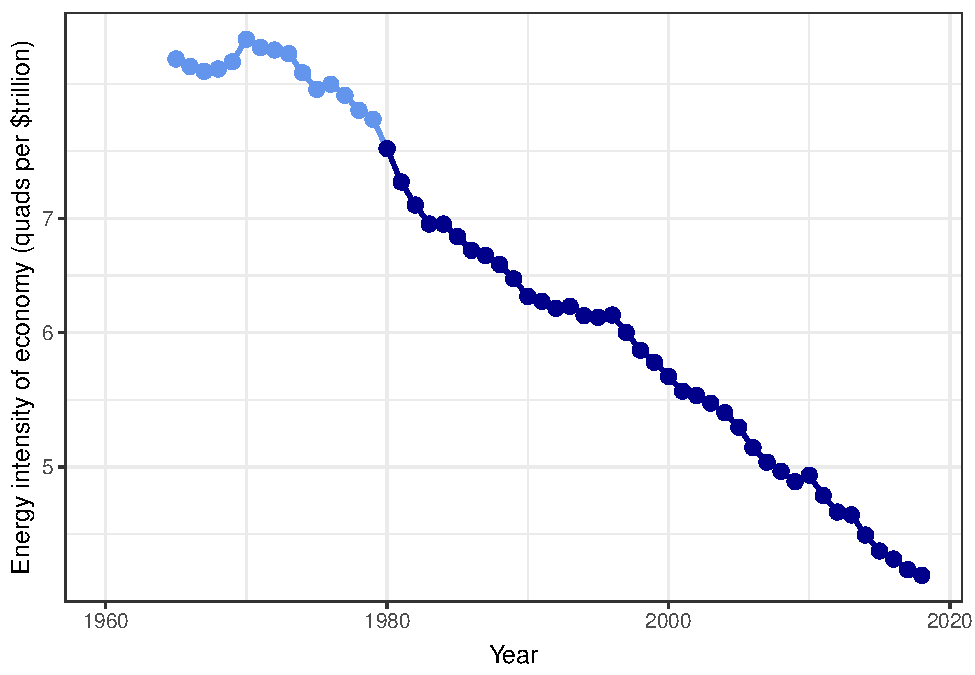
\includegraphics{lab_10_instructions_files/figure-latex/plot_oecd_data-1.pdf}

  Be sure to set \texttt{log\_scale\ =\ TRUE} in the \texttt{plot\_kaya}
  function because a constant percentage rate of change corresponds to a
  linear trend in the logarithm of the variable.
\item
  Next, calculate the rates of change of \emph{P}, \emph{g}, \emph{e},
  and \emph{f} (the Population, per-capita GDP, energy intensity of the
  economy, and carbon-intensity of the energy supply) from your starting
  year through 2018, using the \texttt{lm} function in R.

  A constant rate of change is represented by a linear relationship
  between the natural logarithm of the kaya variable and time: for the
  variable \texttt{P} (population), we would write this formula in R as
  \texttt{log(P)\textasciitilde{}year}.

  Here is an example of calculating the rate of change of \emph{e} (the
  energy intensity of the economy) for the OECD, using the variable
  \texttt{oecd\_data} that you calculated above:

\begin{Shaded}
\begin{Highlighting}[]
\CommentTok{# Load the broom library for organizing lm results}
\KeywordTok{library}\NormalTok{(broom)}
\CommentTok{# Load the magrittr library with helper functions for piping data}
\KeywordTok{library}\NormalTok{(magrittr)}

\NormalTok{e_trend =}\StringTok{ }\NormalTok{oecd_data }\OperatorTok\StringTok{ }\KeywordTok{filter}\NormalTok{(year }\OperatorTok{>=}\StringTok{ }\DecValTok{1980}\NormalTok{) }\OperatorTok
\StringTok{  }\KeywordTok{lm}\NormalTok{(}\KeywordTok{log}\NormalTok{(e) }\OperatorTok{~}\StringTok{ }\NormalTok{year, }\DataTypeTok{data =}\NormalTok{ .) }\OperatorTok
\StringTok{  }\KeywordTok{tidy}\NormalTok{() }\OperatorTok\StringTok{ }\KeywordTok{filter}\NormalTok{(term }\OperatorTok{==}\StringTok{ "year"}\NormalTok{) }\OperatorTok\StringTok{ }\NormalTok{estimate}
\end{Highlighting}
\end{Shaded}

  For more detailed explanation of the code above, see the handout ``New
  Tools for Data Analysis.''

  Here, we find that \texttt{e\_trend} = -0.0141 (-1.41\% per year).

  You can check your results against the interactive web application by
  looking at the rates of change reported on the ``Trends'' tab. Be sure
  to set the start year on the web app to the same values that you used
  for calculating the slopes in RMarkdown.

  These numbers are the slopes of the trend lines that you looked at in
  part 2.
\item
  Using the rates of change that you determined in part 3, use the
  formulas from the ``Growth Rates and Trends'' section to compute the
  values for \emph{P}, \emph{g}, \emph{e}, and \emph{f} in the year
  2050.

  Next, use the growth rates of \emph{P}, \emph{g}, \emph{e}, and
  \emph{f} to calculate the growth rate of the total emissions \emph{F}.
  Calculate the total CO\textsubscript{2} emissions (\emph{F}) from the
  country in 2050, assuming that emissions continue to grow at
  historical rates.

  I recommend that you write R chunks in your report in a way that you
  can copy and paste the chunks from one country or region into the
  analysis for the other countries or regions.

  It may also be useful to define functions for frequently used (e.g.,
  see the example \texttt{growth} function in the handout on ``New Tools
  for Data Analysis'')

  Check your work against the bottom-up numbers in the ``Bottom-Up
  Analysis'' table on the bottom of the left-hand pane of the web
  application.
\item
  Calculate the emissions target for each country: Set the reference
  year for emissions reduction to 2005, and set the target emissions
  reduction using the table below:

  The IPCC developed many representative concentration pathways (RCPs)
  using a top-down approach, for hitting various targets of radiative
  forcing from greenhouse gases. The only RCP that has at least a
  two-thirds probability of keeping warming below 2 degrees Celsius is
  RCP\textasciitilde2.6. This concentration pathway calls for emissions
  reductions (relative to 2005) for different parts of the world listed
  in the table below:

  \begin{longtable}[]{@{}lr@{}}
  \caption{Percent reduction in CO\textsubscript{2} emissions in 2050,
  relative to 2005.}\tabularnewline
  \toprule
  Region & Emissions reduction\tabularnewline
  \midrule
  \endfirsthead
  \toprule
  Region & Emissions reduction\tabularnewline
  \midrule
  \endhead
  Australia/New Zealand & 82\%\tabularnewline
  Canada & 72\%\tabularnewline
  China & 78\%\tabularnewline
  India & 73\%\tabularnewline
  Japan & 66\%\tabularnewline
  South Korea & 67\%\tabularnewline
  United States & 73\%\tabularnewline
  Africa & 28\%\tabularnewline
  Latin America & 40\%\tabularnewline
  Middle East & 32\%\tabularnewline
  Southeast Asia & -17\%\tabularnewline
  Western Europe & 74\%\tabularnewline
  World & 36\%\tabularnewline
  \bottomrule
  \end{longtable}

  Note that Southeast Asia has a negative reduction. This means that
  countries in this region are allowed a 17\% \emph{increase} in
  CO\textsubscript{2} emissions (\emph{F}).

  Set the target year in the web app to 2050; set the reference year to
  2005; set the emissions reduction to the emissions reduction you are
  trying to achieve.

  For each country, how much CO\textsubscript{2} (\emph{F}) would each
  country emit in 2050 in order to meet your policy goal? (Remember to
  work this whole exercise for whole world before starting on the
  individual countries.)

  Let's work an example using the Middle East:

\begin{Shaded}
\begin{Highlighting}[]
\NormalTok{F_}\DecValTok{2005}\NormalTok{_middle_east =}\StringTok{ }\KeywordTok{get_kaya_data}\NormalTok{(}\StringTok{"Middle East"}\NormalTok{) }\OperatorTok\StringTok{ }
\StringTok{  }\KeywordTok{filter}\NormalTok{(year }\OperatorTok{==}\StringTok{ }\DecValTok{2005}\NormalTok{) }\OperatorTok\StringTok{ }\NormalTok{F}
\NormalTok{F_}\DecValTok{2005}\NormalTok{_middle_east}
\end{Highlighting}
\end{Shaded}

\begin{verbatim}
## [1] 1365.124
\end{verbatim}

\begin{Shaded}
\begin{Highlighting}[]
\NormalTok{middle_east_reduction =}\StringTok{ }\FloatTok{0.32}
\NormalTok{F_goal_middle_east =}\StringTok{ }\NormalTok{F_}\DecValTok{2005}\NormalTok{_middle_east }\OperatorTok{*}\StringTok{ }\NormalTok{(}\DecValTok{1} \OperatorTok{-}\StringTok{ }\NormalTok{middle_east_reduction)}
\NormalTok{F_goal_middle_east}
\end{Highlighting}
\end{Shaded}

\begin{verbatim}
## [1] 928.2841
\end{verbatim}

  Check this result against the interactive web application.
\item
  Look up what the CO\textsubscript{2} emission is in 2018 and calculate
  the rate of change in \emph{F} that would be necessary to achieve your
  policy target. For the 2050~calculation:

  \begin{enumerate}
  \def\labelenumii{\alph{enumii}.}
  \tightlist
  \item
    Calculate the ratio of \(F_{2050}/F_{2018}\).
  \item
    Take the natural logarithm of this ratio (in R, the natural
    logarithm function is \texttt{log()}; on your calculator it is
    ``LN'').
  \item
    Divide the logarithm by the number of years (\(2050 - 2018\)). This
    is the rate of change of \emph{F}. A positive number means growth
    and a negative number means a reduction. The percentage rate of
    change per year is 100 times this number.
  \end{enumerate}

  For our Middle East example:

\begin{Shaded}
\begin{Highlighting}[]
\NormalTok{F_}\DecValTok{2017}\NormalTok{_middle_east =}\StringTok{ }\KeywordTok{get_kaya_data}\NormalTok{(}\StringTok{"Middle East"}\NormalTok{) }\OperatorTok\StringTok{ }
\StringTok{  }\KeywordTok{filter}\NormalTok{(year }\OperatorTok{==}\StringTok{ }\DecValTok{2017}\NormalTok{) }\OperatorTok\StringTok{ }\NormalTok{F}
\NormalTok{r_F_middle_east =}\StringTok{ }\KeywordTok{log}\NormalTok{(F_goal_middle_east }\OperatorTok{/}\StringTok{ }\NormalTok{F_}\DecValTok{2017}\NormalTok{_middle_east) }\OperatorTok{/}\StringTok{ }
\StringTok{  }\NormalTok{(}\DecValTok{2050} \OperatorTok{-}\StringTok{ }\DecValTok{2017}\NormalTok{)}
\NormalTok{r_F_middle_east}
\end{Highlighting}
\end{Shaded}

\begin{verbatim}
## [1] -0.02442946
\end{verbatim}

  so total emissions for the Middle East would need to drop by -2.44\%
  per year between 2018 and 2050
\item
  Now calculate the decarbonization rate implied by the policy goal.
  This is the rate of reduction of \emph{ef}, the carbon intensity of
  the economy. \(F = Pgef\), so \(r_F = r_P + r_g + r_e + r_f\).
  Subtract the projected \emph{r\textsubscript{P}} and
  \emph{r\textsubscript{g}} (look them up in the ``Bottom up Analysis''
  table) from \emph{r\textsubscript{F}}, which you just calculated in
  step\textasciitilde7, to get the rate of change of \emph{ef}. Multiply
  the rate of change of \emph{ef} by -1 to get the rate of
  decarbonization (because negative rate of change is a positive rate of
  decarbonization and vice-versa). Multiply by 100 to get the percent
  implied rate of decarbonization.
\item
  How does the implied rate of decarbonization for each nation compare
  to the historical rate of decarbonization (i.e., the trend in
  \emph{ef} reported in the ``Bottom up Analysis'' table)? Which nation
  will have the hardest time meeting this emission goal without damaging
  its economy?
\end{enumerate}

\end{document}
